%equations, bib. \\
\section{State of the art}
There is little literature specifically on the topic of coupled powered systems with elements both above and below the surface of the sea. I have however found bits and pieces that are useful. Primarily the offshore oil and gas industry, as well as general ROV operations are able to help a bit. The main issue with this project is that it is fairly unique. Usually when dealing with ROV operations, the surface vessel is intended to stay stationary for longer periods of time, or the ROV is neutrally buoyant and able to do its work below regardless of what the surface vessel does on the surface. This project deals with a powered non-buoyant ROV which needs to be able to do both large motions to sweep larger areas of seabed, as well as precision work to move in on and pick up litter. This is a unique problem from the literature I have found.

There are several papers discussing for instance the effect of currents on deep-submergence suspended tooling or ROVs used for oil and gas installations that can help. For example, Lian and Sortland 1996 \cite{lian_manoeuvering_1996}. They also performed simulations, however their paper is focused on non-powered remotely operated tooling as opposed to a remotely operated vehicle. Their results can be useful as a kind of sanity check for the results of the simulations of this project, though their working area is down to 1500m below the surface while it's improbable that the Plan Sea project will ever operate below 200m. 

The tether is also a consideration for this project, Chen et al., 2021 \cite{chen_dynamic_2021} discuss the hydrodynamic effects on ROV tethers under complex sea conditions. Whether or not this is useful for this implementation is uncertain, as the tether simulations are all done by the simulation software. Additionally the tethers used for this iteration are likely so small in diameter that their effects in the sea are likely small. It might be possible to expand the tether simulations to include Chen et al.'s findings in future.

Enevoldsen et al., 2018 \cite{enevoldsen_simplified_2018} provide one of the more useful documents on the topic. They discuss a simplified modelling strategy for ROVs to allow for both greater control capabilities and simulated efforts. The state of this project has not used this information, but it will be very helpful in later iterations to expand the accuracy of the simulation for the ROV, both for control purposes and for a more accurate simulation. For instance a model of the vessel can be implemented into the controller so that it's able to act predictively and not just reactively like a PID controller would. Anderlini, Parker and Thomas, 2018 \cite{anderlini_control_2018} discuss control of an ROV carrying an object. They discuss the sudden added mass of the vessel and how to compensate for it from a control perspective, though their paper focuses more on autonomous underwater maintenance vehicles. This paper as well will be very helpful for further implementation work, but has not been used in any great extent here. The Anderlini paper also primarily focuses on self-propelled underwater vehicles, not the externally lifted version that this project considers. Thingstad and Hveding, 1982 \cite{thingstad_nonbuoyant_1982} have a conference paper on non-buoyant ROVs for performing subsea work. On the surface this sounds perfect, but looking into the paper it is more focused on the physical construction of the ROV rather than the control of it. This makes it less helpful for me. Additionally, Thingstad and Hveding's paper is more than 40 years old at time of writing, and applications of control theory, as well as microelectronics and actuators have evolved a lot since then, making what little control they do discuss less useful.

\section{Mathematical basis}
\label{sec:math}
The root problem can be decomposed into equations \ref{eq:usv} and \ref{eq:rov}. They show the forces that impact the momentums of both the surface vessel and the ROV. The forces that have an impact are hydrodynamic forces, such as buoyancy, righting moment etc. The propulsive forces that the vessels' thrusters provide. Environmental forces coming from waves, winds and currents. And finally the force the coupling acts with on each vessel. Do note that though the form of the equations is the same for the surface vessel and the ROV, the values both in total and in each individual element are not necessarily equal. Hydrodynamic, propulsive and environmental forces will be entirely individual for each element because of their physical shape and capabilities, and while the coupling forces are linked, their relationship is not necessarily linear. See \cref{sec:catenary} for elaboration.

\begin{align}
M_{v_{\text{surf}}} = \sum f &= f_{hydro} + f_{prop} + f_{env} + f_ {coupling} \label{eq:usv}\\
M_{v_{\text{ROV}}} = \sum g &= g_{hydro} + g_{prop} + g_{env} + g_ {coupling} \label{eq:rov}
\end{align}

The equations demonstrate the need for simulation compared to analytical examination of the problem. Hydrodynamic forces and environmental forces contribute to a highly dynamic system for which it is difficult or impossible to find a closed form expression. This means that calculating an expected state for the dynamic system manually is labour and time intensive. Using a simulation instead of analytical methods hides these problems away. The simulation will take care of the complex interactions which allows me to focus on extracting interesting data. I will further discuss simulation options in \cref{sec:sim_options}

Using a simulation does introduce a new requirement: that of validating the models' accuracy. There are many ways of doing this, both intuitively and mathematically. I will get talk more about the validation methods I've chosen in \cref{sec:validation}. 

The simulation allowing for "setting and forgetting" whatever parts of the force equations are desired allows the user to focus on whatever specific field they are interested in. For example a user might examine the propulsive force required given a certain seastate, or how hull shape and hydrodynamics affects the stability of the total system. Using simulation gives the user a greater degree of freedom in finding exactly the variables they're interested in.

\subsection{Catenaries}
\label{sec:catenary}
When a rope or chain is suspended from two points and affected by forces not in-line with the two points, the chain forms a catenary. Catenaries are relevant to this project because the lifting tether will form a catenary whenever the ROV is not directly underneath the surface vessel and also not experiencing any external forces. If there is a current or movement affecting the tether it will form a catenary. 

\begin{figure}
	\centering
	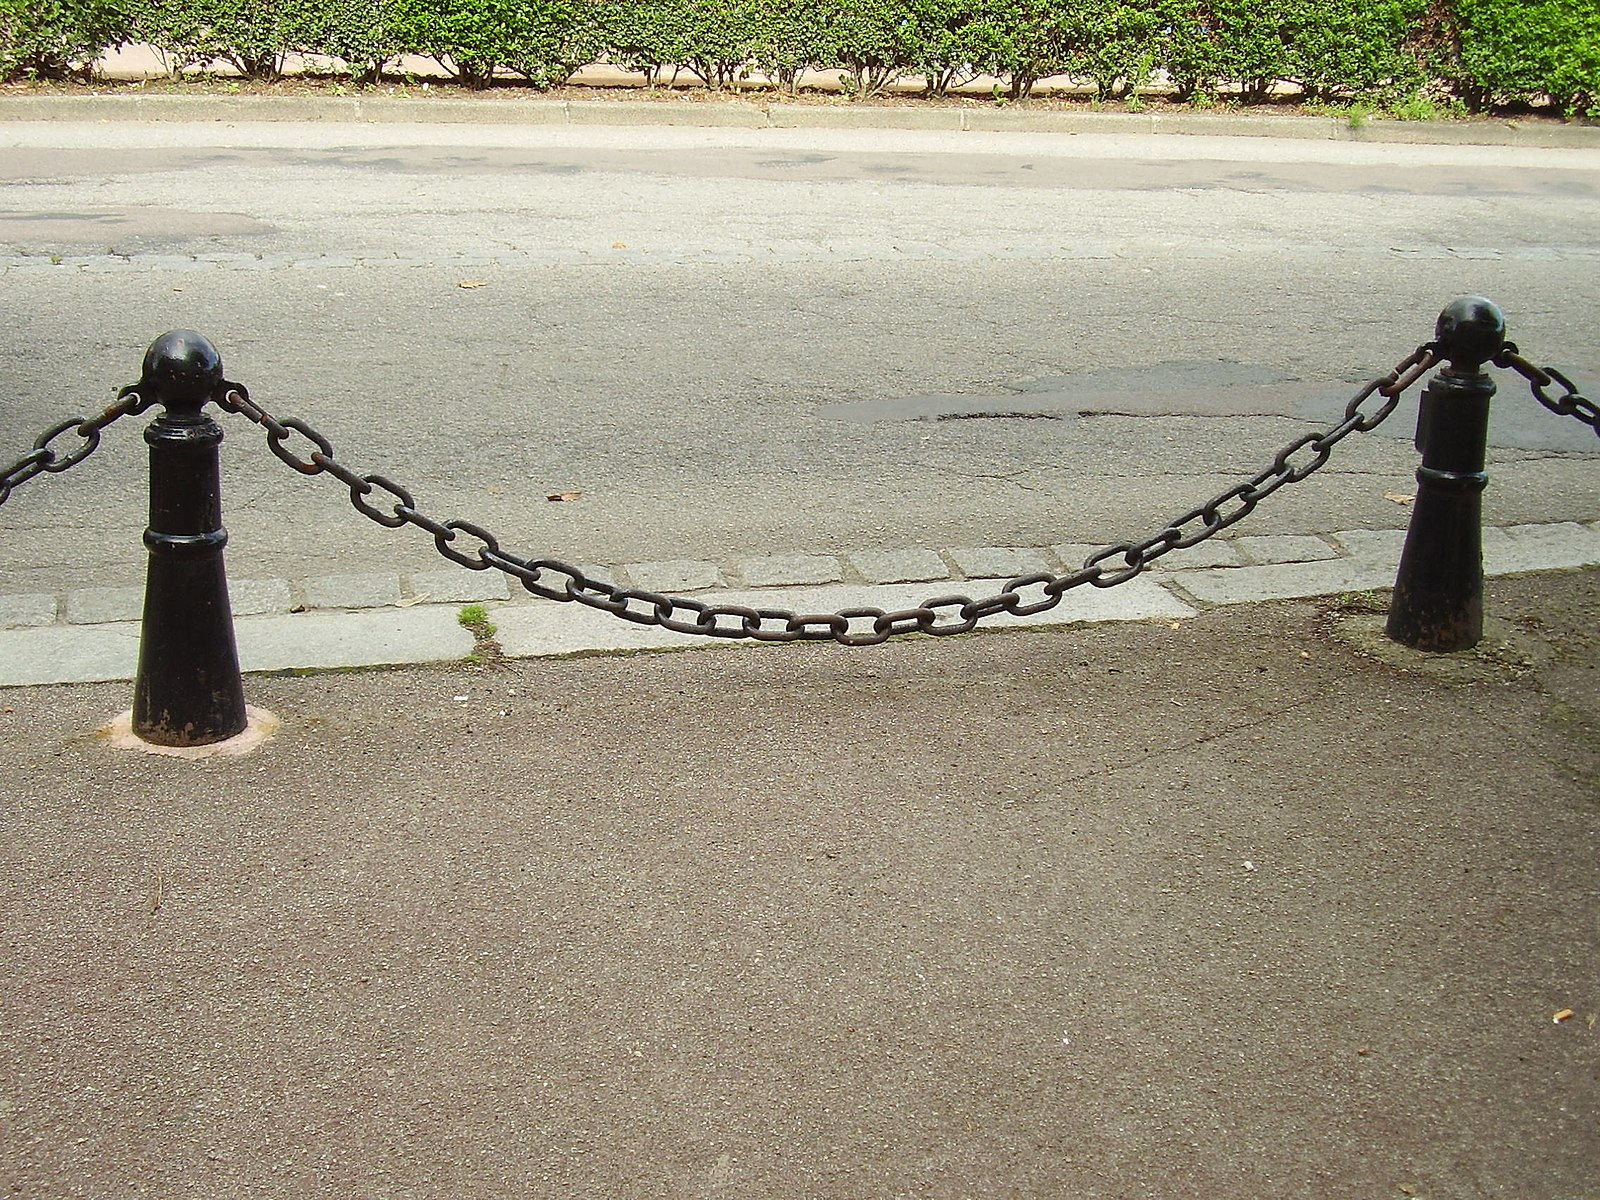
\includegraphics[width=0.8\textwidth]{catenary}
	\caption{Illustration image of a chain forming a catenary between two posts under the force of gravity.\\\scriptsize{Used under Creative Commons, credit: \texttt{https://en.wikipedia.org/wiki/File:Kette\_Kettenkurve\_Catenary\_2008\_PD.JPG}}}
	\label{fig:catenary}
\end{figure}

The fact that the lifting tether will form a catenary is helpful to know, as one might intuitively assume that the lifting tether would be straight between the surface vessel and the ROV. If the tether were smooth, finding the position of the ROV could be done by trigonometry, knowing the length of the tether, its angle at the lifting point relative to gravity, and knowing the tether's azimuth, the ROV could be located using Pythagoras' theorem. However, since this simplification can't necessarily be done, a slight complication has to be added. The angle at the lifting point is not necessarily directly linked to the angle of a straight line to the ROV. This can be seen demonstrated in \cref{fig:notstraight}

\begin{figure}
	\centering
	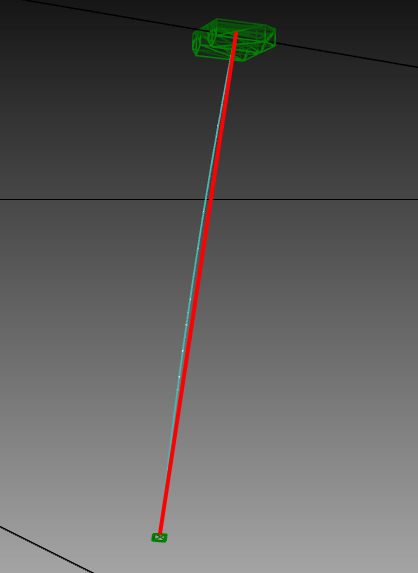
\includegraphics[width=0.8\textwidth]{notstraight}
	\caption{The simulation showing the towing line (light blue) and a straight line between the surface vessel and the ROV (red). Note how the towing line is not straight}
	\label{fig:notstraight}
\end{figure}

In 2 dimensions, a catenary is well defined as 
\[y = a \cosh\left(\frac x a \right)\] 
Where \(a\) defines the width of the catenary and can be found in relation to the relevant forces acting on the rope. For this project's applications however, the shape of the tether can't necessarily be simplified to 2D. I have been unable to find a simple, closed form of the catenary equation in 3D for a rope (as opposed to a plane), though it may well exist. This further solidifies the necessity of a simulation over using analytical methods. Additionally, the simulator has shown that the tether does not necessarily form a catenary. This is also shown in \cref{fig:notstraight} where the shape of the tether is more bowed near the surface than near the bottom.

This simulator can be used to find an error between assuming a straight line between the ROV and the surface vessel, compared to the real situation. This relationship or error can be included as a part of the internal model of the vessel's state estimator and  be used as a part of positioning the ROV under water. 
